\documentclass{article}%
\usepackage[T1]{fontenc}%
\usepackage[utf8]{inputenc}%
\usepackage{lmodern}%
\usepackage{textcomp}%
\usepackage{lastpage}%
\usepackage{authblk}%
\usepackage{graphicx}%
%
\title{MMP7{-}mediated cleavage of nucleolin at Asp255 induces MMP9 expression to promote tumor malignancy}%
\author{Nancy Allen}%
\affil{The Johns Hopkins Oncology Center, Program in Human Genetics, and The Howard Hughes Medical Institute, The Johns Hopkins University School of Medicine, 424 N. Bond Street, Baltimore, 21231, Maryland, USA}%
\date{01{-}01{-}2006}%
%
\begin{document}%
\normalsize%
\maketitle%
\section{Abstract}%
\label{sec:Abstract}%
STAT1 and STAT3 phosphorylation by porins are independent of JAKs but are dependent on MAPK pathway and plays a role in U937 cells production of interleukin{-}6, a new cell signaling cell signaling protein described in a special study published online by the journal Science.\newline%
JAKs are unique individual molecules that play a variety of roles in many cell signaling processes, such as mitochondrial and fibroblast cell division, cell signaling and the production of multiple signaling proteins. Although there are four versions of JAK, including an ADK (additional form of ADK), the researchers at Joslin Diabetes Center, Boston, discovered that STAT1 and STAT3 phosphorylation differs from BAC (required) to make U937 cells.\newline%
Our results suggest that STAT1{-}STAT3 phosphorylation may play a role in U937s production of interleukin{-}6 but does not explain its role in cell proliferation, said Jennifer Prato, MD, a senior author of the Science study and an associate professor of internal medicine at Joslin Diabetes Center.\newline%
Stat3 phosphorylation accounts for a type of enzyme deficiency that occurs in an abundance of U937 cell signaling proteins. U937 helps normalize the metabolism of waste products, solid and liquid waste, and prevent damage to cell membranes. Because U937 plays an important role in such processes, STAT3 phosphorylation and its function can be carried out independently of other JAKs and STAT2 and STAT3 phosphorylation in U937 cells.\newline%
Our findings suggest that STAT3 phosphorylation differs from BAC in the majority of U937 cells and that these cells may have different phosphorylation requirements for different types of cell signaling, said author Antonio J. G. Zammitrova, MD, of the Department of Surgery at Joslin Diabetes Center.\newline%
The researchers found that STAT3 phosphorylation is related to the complement blockade of an important functional protein called interleukin{-}6 (IL{-}6). The formation of activated U937 cells reduces the uptake of IL{-}6 by the ligand IL{-}1. When other receptors for D2, IL{-}3, and IL{-}4 are added, this blocking of IL{-}1 leads to the breakdown of the interleukin{-}6 protein and the formation of many mediators of stem cell proliferation.\newline%
The group noted that it must be clarified how STAT3 regulates U937s signaling to produce interleukin{-}6, which for patients with aggressive and cancerous types of U937 begins with the progression of their disease.\newline%
The full study can be viewed at http://bios.sys.state.ma.us.\newline%
Visit the Stanford University School of Medicine Web site ( www.stanford.edu/resources/med/brittlepackets/index.asp) for more information about Stanford University medical schools.

%
\subsection{Image Analysis}%
\label{subsec:ImageAnalysis}%


\begin{figure}[h!]%
\centering%
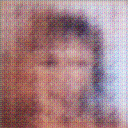
\includegraphics[width=150px]{500_fake_images/samples_5_238.png}%
\caption{A Close Up Of A Black And White Cat}%
\end{figure}

%
\end{document}